\documentclass[final,dvipsnames]{beamer}
\usepackage{amsmath,amsfonts,amssymb,pxfonts,eulervm,xspace}
\usepackage{graphicx,subfigure,comment,tikz}
\usepackage{array}
\usepackage{adjustbox}
\usepackage{framed}
\usepackage{xcolor}
\usepackage{mdframed}
\usepackage{multirow}
\usepackage{svaiter}
\usepackage[utf8]{inputenc}
\usepackage{arydshln}
\usepackage{relsize}
\usepackage{ragged2e}

\graphicspath{{./img/}}
\usepackage[orientation=landscape,size=a0,scale=1.5,debug]{beamerposter}

\mode<presentation>{\usetheme{inriaposter}}

\makeatletter
\pgfkeys{/pgf/.cd,
  parallelepiped offset x/.initial=2mm,
  parallelepiped offset y/.initial=2mm
}
\pgfdeclareshape{parallelepiped}
{
  \inheritsavedanchors[from=rectangle] % this is nearly a rectangle
  \inheritanchorborder[from=rectangle]
  \inheritanchor[from=rectangle]{north}
  \inheritanchor[from=rectangle]{north west}
  \inheritanchor[from=rectangle]{north east}
  \inheritanchor[from=rectangle]{center}
  \inheritanchor[from=rectangle]{west}
  \inheritanchor[from=rectangle]{east}
  \inheritanchor[from=rectangle]{mid}
  \inheritanchor[from=rectangle]{mid west}
  \inheritanchor[from=rectangle]{mid east}
  \inheritanchor[from=rectangle]{base}
  \inheritanchor[from=rectangle]{base west}
  \inheritanchor[from=rectangle]{base east}
  \inheritanchor[from=rectangle]{south}
  \inheritanchor[from=rectangle]{south west}
  \inheritanchor[from=rectangle]{south east}
  \backgroundpath{
    % store lower right in xa/ya and upper right in xb/yb
    \southwest \pgf@xa=\pgf@x \pgf@ya=\pgf@y
    \northeast \pgf@xb=\pgf@x \pgf@yb=\pgf@y
    \pgfmathsetlength\pgfutil@tempdima{\pgfkeysvalueof{/pgf/parallelepiped offset x}}
    \pgfmathsetlength\pgfutil@tempdimb{\pgfkeysvalueof{/pgf/parallelepiped offset y}}
    \def\ppd@offset{\pgfpoint{\pgfutil@tempdima}{\pgfutil@tempdimb}}
    \pgfpathmoveto{\pgfqpoint{\pgf@xa}{\pgf@ya}}
    \pgfpathlineto{\pgfqpoint{\pgf@xb}{\pgf@ya}}
    \pgfpathlineto{\pgfqpoint{\pgf@xb}{\pgf@yb}}
    \pgfpathlineto{\pgfqpoint{\pgf@xa}{\pgf@yb}}
    \pgfpathclose
    \pgfpathmoveto{\pgfqpoint{\pgf@xb}{\pgf@ya}}
    \pgfpathlineto{\pgfpointadd{\pgfpoint{\pgf@xb}{\pgf@ya}}{\ppd@offset}}
    \pgfpathlineto{\pgfpointadd{\pgfpoint{\pgf@xb}{\pgf@yb}}{\ppd@offset}}
    \pgfpathlineto{\pgfpointadd{\pgfpoint{\pgf@xa}{\pgf@yb}}{\ppd@offset}}
    \pgfpathlineto{\pgfqpoint{\pgf@xa}{\pgf@yb}}
    \pgfpathmoveto{\pgfqpoint{\pgf@xb}{\pgf@yb}}
    \pgfpathlineto{\pgfpointadd{\pgfpoint{\pgf@xb}{\pgf@yb}}{\ppd@offset}}
  }
}
\makeatother

%-- Header and footer information ----------------------------------
\newcommand{\footleft}{\footnotesize hashem.ghanem@grenoble-inp.fr, nicolas.keriven@grenoble-inp.fr, nicolas.tremblay@grenoble-inp.fr}
\newcommand{\footright}{\footnotesize This work was supported by ANR GraVa ANR-18-CE40-0005 and ANER RAGA G048CVCRB2018ZZ.}
\title{Fast graph kernel with optical random features}
\author{ \qquad Hashem Ghanem\qquad Nicolas Keriven \qquad Nicolas Tremblay}
\institute{GIPSA-lab, CNRS, UGA, Grenoble INP, France
}
\newcommand{\vsp}{\vspace{10pt}}
\newcommand{\vspp}{\vspace{-10pt}}
\usetikzlibrary{arrows.meta}
%-------------------------------------------------------------------

\newcommand{\cita}[1]{{\footnotesize \emph{(#1)}}}

\newcommand{\myemph}[1]{\textcolor{red}{#1}}
\newcommand{\myemphh}[1]{\textbf{\textcolor{red}{#1}}}
\newcommand{\mycolbacksum}[1]{
\hspace*{.01\linewidth}\begin{minipage}{.96\linewidth}
\begin{mdframed}[backgroundcolor=blue!10,linewidth=0pt]
\vsp
#1
%\vsp
\end{mdframed}
\end{minipage}
}
\newcommand{\mycolback}[1]{
\hspace*{.01\linewidth}\begin{minipage}{.96\linewidth}
\begin{mdframed}[backgroundcolor=blue!10,linewidth=0pt]
\vsp
#1
\vsp
\end{mdframed}
\end{minipage}
}
\newcommand{\mycolbackk}[1]{
\hspace*{.01\linewidth}\begin{minipage}{.96\linewidth}
\begin{mdframed}[backgroundcolor=red!10,linewidth=0pt]
\vsp
#1
\vsp
\end{mdframed}
\end{minipage}
}
\newcommand{\mycolbackwhite}[1]{
\hspace*{.01\linewidth}\begin{minipage}{.96\linewidth}
\begin{mdframed}[backgroundcolor=white,linewidth=1pt]
\vsp
#1
\vsp
\end{mdframed}
\end{minipage}
}
\usetikzlibrary{decorations.pathreplacing}

\begin{document}
\begin{frame}{}
\vspace{-40pt}
\begin{columns}[t]
%%%%%%%%%%%%%%%%%%%%%%%%%%%%%%%%%%%%%%%%%%%%%%%%%%%%%%%%%%%%%%%%%%%%%%%%%%%%%%%%%
\begin{column}{0.25\linewidth}
\begin{myalertblock}{1: Summary}
	The \textbf{graphlet kernel}is a classical method in graph classification. It however suffers from a high computation cost due to the isomorphism test it includes.  
\begin{center}	
\mycolbacksum{We propose to leverage \myemph{kernel random features} within the graphlet framework, and establish a theoretical link with the \myemph{MMD metric}. If this method can still be prohibitively costly for usual random features, we then incorporate \myemph{optical} random features that can be computed in \emph{constant time}.}
\end{center}

\end{myalertblock}
\vsp 


\begin{myalertblock}{3: Efficiency of $GSA-\varphi$ with  $\varphi_{RF}$ \emph{w.r.t.} the \myemph{MMD} metric.}
\vspace{0.3cm}
\small 
\begin{itemize}
	\item $\kappa(\mathbf{x},\mathbf{x}')= \mathbb{E}_{\mathbf{w} \sim p}~ \xi_\mathbf{w}(\mathbf{x})^* \xi_\mathbf{w}(\mathbf{x}')$ (kernels with RFs).
	\vsp
	\item $\varphi_{RF}(\mathbf{x}) = \frac{1}{\sqrt{m}} ( \xi_{\mathbf{W}_j}(\mathbf{x}) )_{j=1}^m \Rightarrow\kappa(\mathbf{x},\mathbf{x}')\approx \varphi_{RF}(\mathbf{x})^*\varphi_{RF}(\mathbf{x}')$
	\vsp 
	\item  $\kappa_{GS}(\mathbf{x},\mathbf{x}')=\exp^{-\frac{\left \| \mathbf{x}-\mathbf{x}'\right\|^2}{2\sigma^2}} \Rightarrow \varphi_{GS}(\mathbf{x}) = \frac{\sqrt{2}}{\sqrt{m}} cos( \mathbf{W}^T\mathbf{x}+b )$

\end{itemize}
\vsp
\mycolback{
\textbf{Theorem}
Let $\mathcal{G}$ and $\mathcal{G}'$ be two graphs.  Assume that $|\xi_\mathbf{w}(F)| \leq 1$.
Then, for all $\delta>0$, with probability at least $1-\delta$:
\begin{align*}
	\Big|\textcolor{red}{\|\mathbf{z}_\mathcal{G} - \mathbf{z}_{\mathcal{G}'}\|^2 - MMD(\mathbf{f}_\mathcal{G},\mathbf{f}_{\mathcal{G}'})^2} \Big| \leq \\\frac{4 \sqrt{\log (6/\delta)}}{\sqrt{m}} + \frac{8\left(1+\sqrt{2\log(3/\delta)}\right)}{\sqrt{{s}}}
\end{align*}
}
\vspace{1cm}
\end{myalertblock}

\begin{myalertblock}{4: Incorporating \myemph{Optical random featurs}}
	\vspace{0.3cm}
	\mycolback{
		\begin{itemize}
			\item  ${\varphi}_{OPU}(\mathbf{x})=|\mathbf{Wx+b}|^2 ;~\mathbf{W}\in \mathbb{R}^{m\times d}, \mathbf{x}\in \mathbb{R}^d$
			\vsp
			\item  $m\mapsto\infty \Rightarrow$\\ 
			$\quad {\varphi}_{OPU}(\mathbf{x_1})^T{\varphi}_{OPU}(\mathbf{x_2})\approx \kappa_{OPU}(\mathbf{x_1}, \mathbf{x_2})$
			\vsp
			\item \myemph{Optical Processing Units (OPUs)} evaluate $\varphi_{OPU}$ in \myemph{$\mathcal{O} (1)$} in both input/output dimensions $(d,m)$.
		\end{itemize}
		
	}
  \begin{center}
  \includegraphics[width=0.7\linewidth]{figs/opu}
\end{center}
\end{myalertblock}

\end{column}%1




%%%%%%%%%%%%%%%%%%%%%%%%%%%%%%%%%%%%%%%%%%%%%%%%%%%%%%%%%%%%%%%%%%%%%%%%%%%%%%%%%%%%%%%%%%%%%%
\begin{column}{0.45\linewidth}

\begin{block}{2: From the graphlet kernel to \myemph{$GSA-\varphi$}}
	\hspace*{.0\linewidth}\begin{minipage}{.99\linewidth}
		
		\begin{center}
			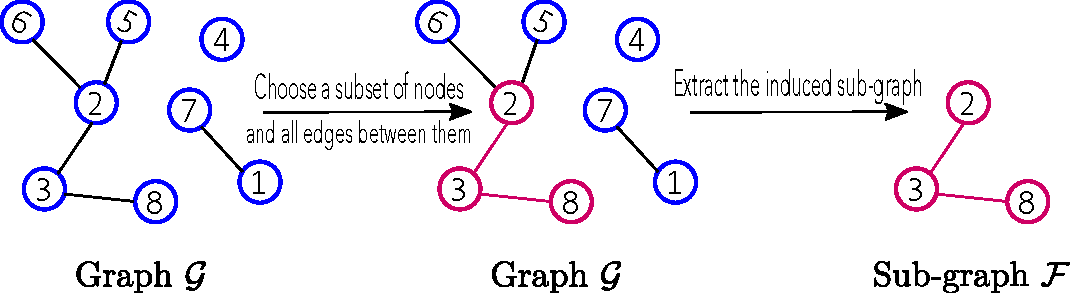
\includegraphics[height=10cm]{figs/subgraphs.pdf}
		\end{center}
	
		\begin{mynotablock}
			\vsp
			\parbox{0.4\textwidth}{
				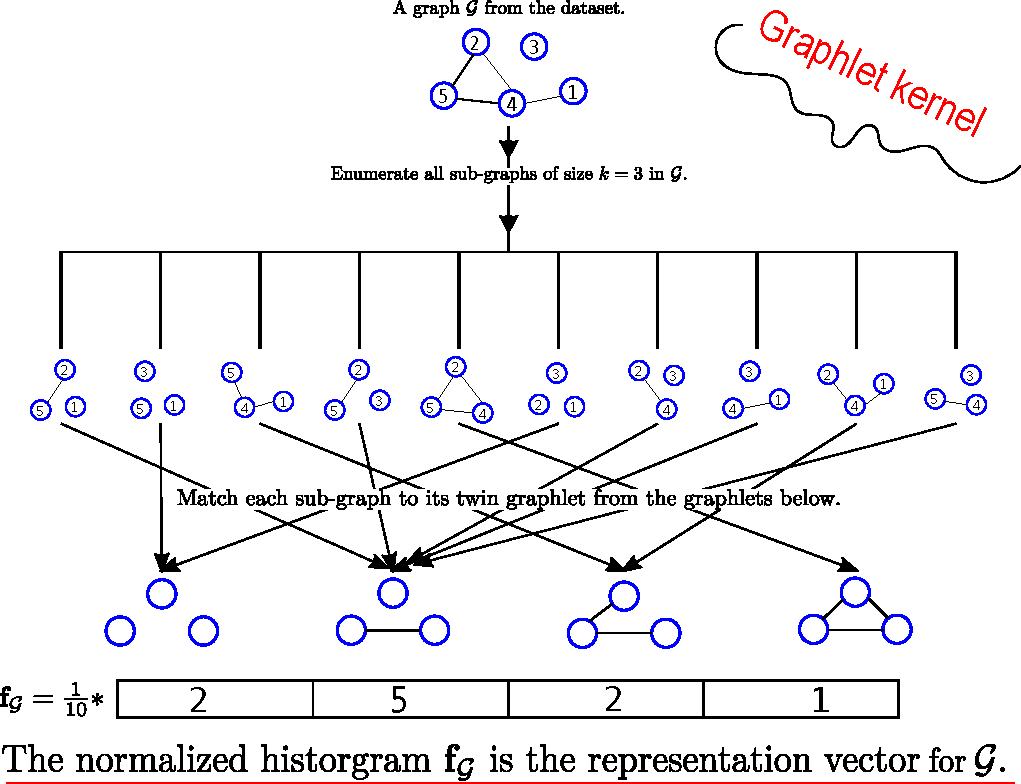
\includegraphics[height=25cm]{figs/gk.pdf}
			}
			\hfill
			\parbox{0.35\textwidth}{
				\large
				\begin{itemize}
					\item  \myemph{Exp. cost}:  $O\big(\tbinom{v}{k} N_k C^{\cong}_k\big)$
					\vsp
					\item Can be a bit reduced: $O(\textcolor{red}{s}N_k C^{\cong}_k)$
					\vsp
					\item Still \myemph{exponential}.
				\end{itemize}
			}
		
		\end{mynotablock}
	\end{minipage}

\vspace{1cm}
\begin{itemize}
	\item Replace the matching with \myemph{$\varphi:$ \{size-$k$ subgraphs\} $\mapsto\mathbb{R}^m$}
\end{itemize}
\vspace{1cm}
\parbox{0.4\textwidth}{
	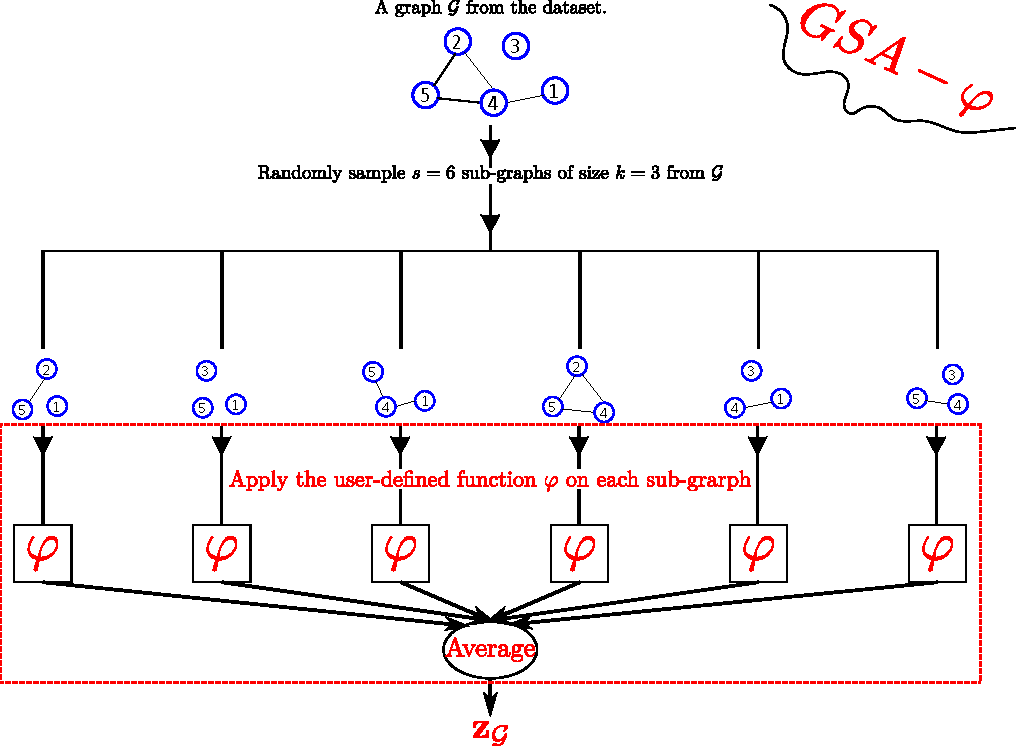
\includegraphics[height=25cm]{figs/GSA_phi.pdf} 
}
\hfill
\parbox{0.35\textwidth}{
	\large
	\begin{itemize}
		\item  Gen. cost: $O(s C_{\varphi})$
		\vsp
		\item \textbf{Gaussian} map: $O(s m k^2)$
		\vsp
		\item \myemph{OPU map: $O(s)$}
	\end{itemize}
}

\vspace{1cm}
\large
\hspace {12cm}\myemph{$\mathbf{z}_\mathcal{G}$ }represents $\mathcal{G}$.
\end{block}

\end{column}








%%%%%%%%%%%%%%%%%%%%%%%%%%%%%%%%%%%%%%%%%%%%

\begin{column}{0.29\linewidth}
	
	
\begin{myalertblock}{5: Experiments}
\vspace{0.5cm}

\hspace*{.0\linewidth}\begin{minipage}{.99\linewidth}
	\begin{mynotablock}{\textbf{$GSA-\varphi_{OPU}$ Vs. graphlet kernel and GCNs}}
		\small
		\begin{itemize}
			\item Dataset: 300 graphs based on the stochastic block model.
			\item Lft: $GSA-\varphi_{OPU}$ with uniform sampling. 
			\item Rgt: $GSA-\varphi_{OPU}$ with random walks, graphlet kernel, and GIN model.
			\item If not mentioned: $s= 2000, m=5000$.
			
		\end{itemize}
		\vsp
		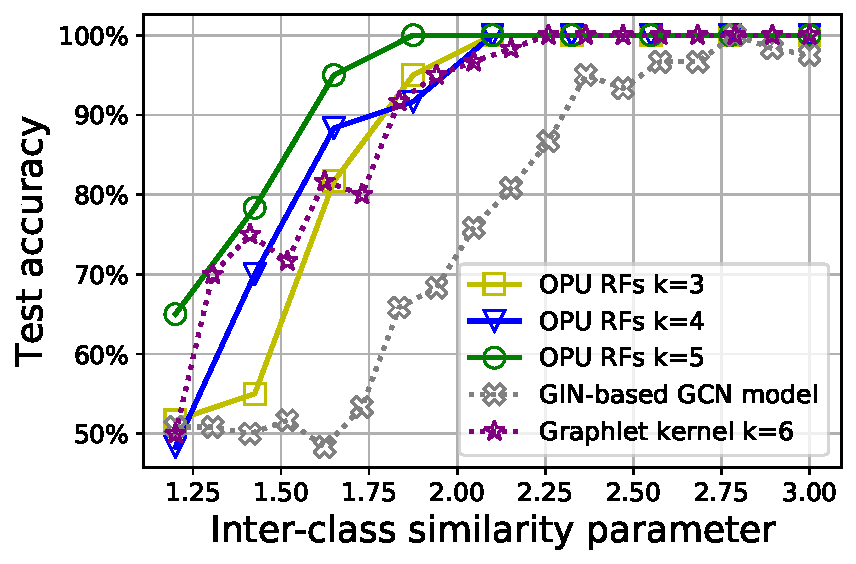
\includegraphics[width=0.45\linewidth]{figs/LightOn_adj_SBM_similarity_graphlet_size_RW.pdf}\hfill
		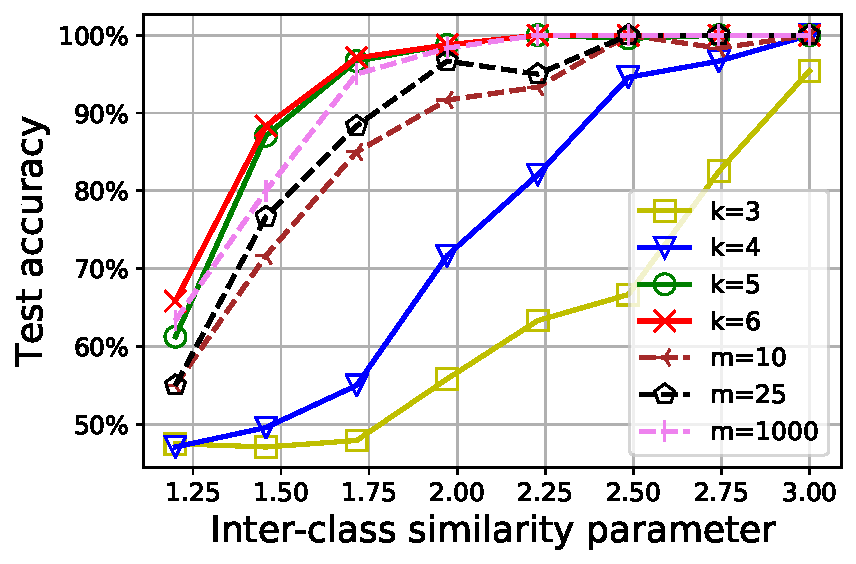
\includegraphics[width=0.45\linewidth]{figs/LightOn_adj_SBM_Similarity_graphlet_size.pdf}		
	\end{mynotablock}
\end{minipage}
\vspace{0.5cm}

\hspace*{.0\linewidth}\begin{minipage}{.99\linewidth}
	\begin{mynotablock}{\textbf{$GSA-\varphi$ with different $\varphi_{RF}$ + comp. cost}}
		\small 
		\begin{itemize}
			\item $s=2000, m = 5000$.
		\end{itemize}
		\vsp
		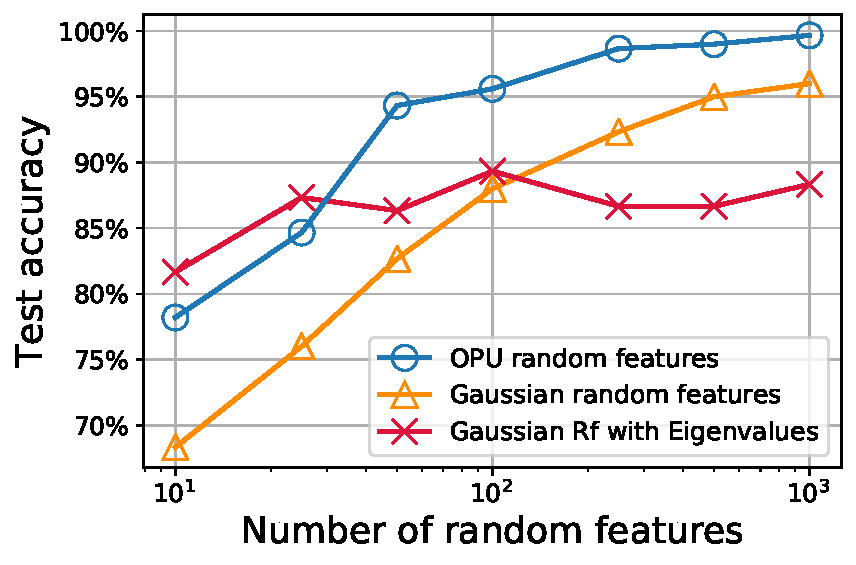
\includegraphics[width=0.45\linewidth]{figs/phi_comparison.pdf}\hfill
		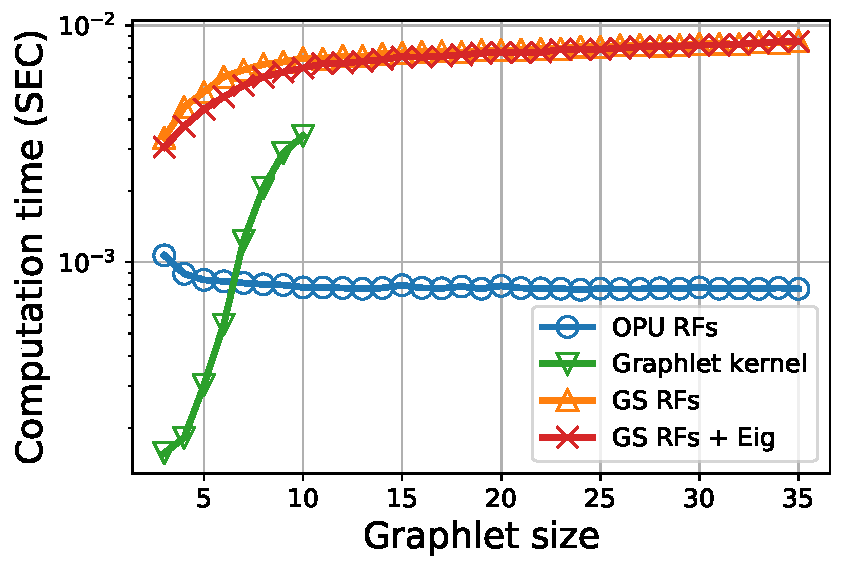
\includegraphics[width=0.45\linewidth]{figs/computational_comp.pdf}		
	\end{mynotablock}
\end{minipage}
\vspace{0.5cm}

\hspace*{.0\linewidth}\begin{minipage}{.99\linewidth}
\begin{mynotablock}{\textbf{Results on real world datasets.}}
	\small 
	\begin{itemize}
		\item Lft: D\&D dataset, rgt: Reddit-Binary. ($s=2000, m = 5000$).
	\end{itemize}
	\vsp
	 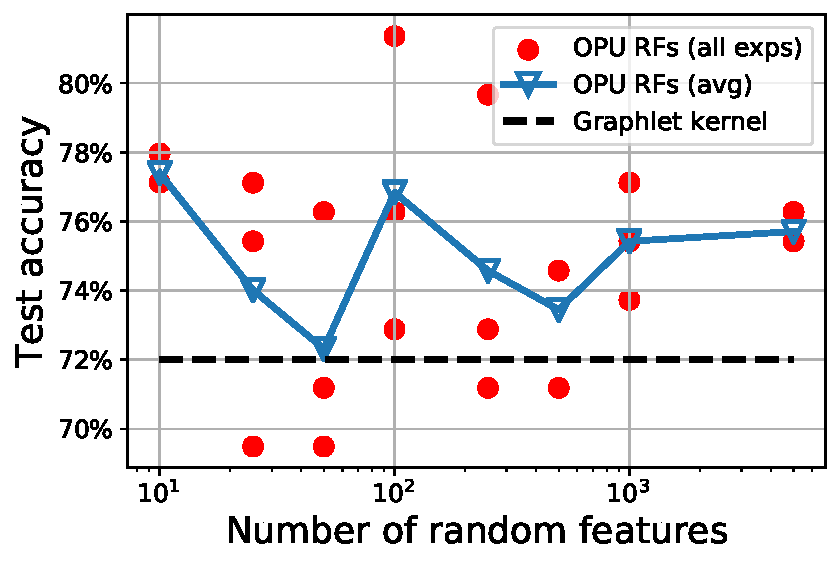
\includegraphics[width=0.45\linewidth]{figs/DD.pdf}\hfill
	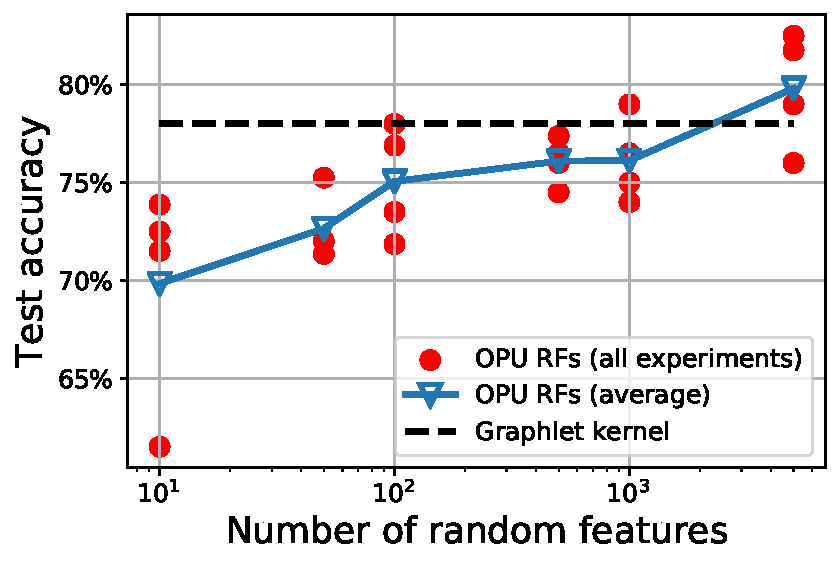
\includegraphics[width=0.45\linewidth]{figs/Reddit.pdf}

\end{mynotablock}
\end{minipage}
\end{myalertblock}


 {\footnotesize
   \begin{itemize}
   \item[{[1]}]Saade et al. \textbf{Random projections through multiple optical scattering: Approximating kernels at the speed of light}. \emph{ICASSP}, 2016.
   \item[{[2]}] Shervashidze et al. \textbf{Efficient graphlet kernels for large graph comparison}. \emph{International Conference on Artificial Intelligence and Statistics}, 2009.
    \item[{[3]}] Rahimi et al. \textbf{Random features for large-scale kernel machines}. \emph{NIPS}, 2007.

	
\end{itemize}
 }

% \end{block}%2


\end{column}
\end{columns}




\end{frame}
\end{document}
